\section{Preliminaries and Notation}
\label{intro:preliminaries_notation
}

We consider a $y$--invariant, doubly layered structure
with a periodic interface separating two materials; see Figure 2.
\vspace{-14mm}
%
% Figure: Geometry
%
\begin{figure}[H]
\begin{center}
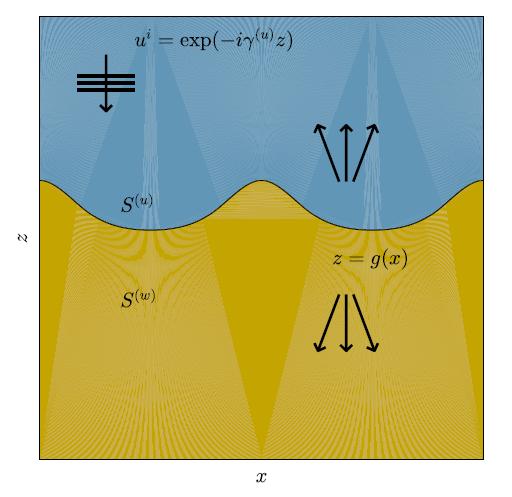
\includegraphics[width=80mm]{figures/two_layer_interface.png}
\caption{A two-layer structure with a periodic interface,
    $z=g(x)$, separating two material layers, $S^{(u)}$ and
    $S^{(w)}$, illuminated by plane--wave incidence.}
\end{center}
\end{figure}
\vspace{-22mm}
The $d$--periodic interface shape is specified by the graph of the function
$z = g(x)$, $g(x+d) = g(x)$. A dielectric (with refractive index $n^u$) 
occupies the domain above the interface
$$
S^{(u)} := \{ z > g(x) \},
$$
while a material of refractive index $n^w$ is in the lower layer
$$
S^{(w)} := \{ z < g(x) \}.
$$
The subscripts are chosen to conform to the notation of
\cite{Nicholls12,Nicholls17}.
The structure is illuminated from above by monochromatic plane--wave incident radiation
of frequency $\omega$ and wavenumber $k^u = n^u\omega/c_0=\omega/c^u$ 
($c_0$ is the speed of light) aligned with the grooves
$$
\textbf{\underline{E}}^{\text{inc}}(x,z,t) = \textbf{A} e^{-i \omega t + i \alpha x - i \gamma z},
\quad
\textbf{\underline{H}}^{\text{inc}}(x,z,t) = \textbf{B} e^{-i \omega t + i \alpha x - i \gamma z}.
$$
We consider the reduced incident fields

\begin{gather*}
\textbf{E}^{\text{inc}}(x,z) = e^{i \omega t} \textbf{\underline{E}}^{\text{inc}}(x,z,t),
\quad
\textbf{H}^{\text{inc}}(x,z) = e^{i \omega t} \textbf{\underline{H}}^{\text{inc}}(x,z,t), \\
\alpha := k^u \sin(\theta),
\quad
\gamma^u := k^u \cos(\theta),
\end{gather*}
where the time dependence $\exp(-i\omega t)$ has been factored out. 
As shown in \cite{Petit80}, the reduced electric and magnetic fields
$\{\textbf{E},\textbf{H}\}$ are $\alpha$--quasiperiodic like the incident radiation.
To close the problem we specify that the scattered radiation is ``outgoing,'' 
upward propagating in $S^{(u)}$ and downward propagating in $S^{(w)}$.

It is well known (see, e.g., $\S 1.5-\S 1.7$ and Petit \cite{Petit80}) that in this 
two--dimensional setting, the time--harmonic Maxwell equations decouple into two 
scalar Helmholtz problems which govern the Transverse Electric and 
Transverse Magnetic polarizations. We define the invariant ($y$) direction
of the scattered (electric or magnetic) fields by $\tilde{u} = \tilde{u}(x,z)$
and $\tilde{w} = \tilde{w}(x,z)$ in $S^{(u)}$ and $S^{(w)}$, respectively. The incident radiation in the upper field is defined as $\tilde{u}^i(x,z)$ (which we will also denote by $\tilde{u}^{inc}(x,z))$. In Chapters $2$ and $3$ we will factor out the phase
$\exp(i \alpha x)$ from the fields $\tilde{u}$ and $\tilde{w}$
$$
u(x,z) = e^{-i \alpha x} \tilde{u}(x,z),
\quad
w(x,z) = e^{-i \alpha x} \tilde{w}(x,z),
$$
which, we note, are $d$--periodic. This will simplify notation and, as discussed in  Chapters $2$ and $3$, also remove the phase from the relevant quantities in our governing equations.